%! TEX root = 'main.tex'
\section{Overview}
\label{sec:implant-overview}


Critical infrastructure such as power grids comprises physical and cyber systems and assets that vital to national security. Their failure or incapacity would have a significant impact on people's daily life on a large scale. The recent Ukrainian power grid attack, the massive blackout in south American countries~\cite{haes2019survey} demonstrated that influence not only affects people's livelihoods but even international politics. The cyberattack on the ICS system can even cause physical damage to the infrastructure~\cite{zeller2011myth}, which makes it harder to recover. Incidents such as the Stuxnet proved this point.

Consequently, ICS has received considerable attention due to security concerns. There are many ways to breach a computer system, and most of them are focus on software-based approaches such as vulnerability hunting and exploiting, cracking of authentication and protocols. Therefore, the attacker needs to break into the network and avoid existing access control and other mitigations. Moreover, most critical infrastructures use their air-gapped network, and It may take a state-sponsored team to accomplish such as mission ~\cite{langner2011stuxnet}. 

Under such circumstances, we believe that cyber-attacks with the assistance of physical approaches are underestimated, especially before the emergence of the so-called supply-chain attacks. Among those world-class attacks, the term APT(Advanced Persistent Threat) is often mentioned. In essence, the APT attack is an extremely well-hidden trojan that can be deployed for many years without being detected. Thus, installing the trojan and remotely triggering it is the crucial point of a successful attack.

In this paper, we provide two plans for physically installing a trojan and provide a prototype hardware implant \name that can be used for this type of attack. ~\autoref{fig:bigpic} depict the scenario. In many parts of the supply chain, such as the factory and shipment, numerous employees have the opportunity to access the PLC. Installing an extra piece of a circuit board is not a difficult task for professionals. Moreover, a large-scale infrastructure such as a power grid has many remote substations with very few staff. An attacker can sneak into one of the substations and install the hardware backdoor. The difficulty between the targeted PLC and the attacker, in reality, can be just a few padlocks. We believe that the breach of a substation can cause a chain reaction in a power grid, and it is a real threat~\cite{substationattack}~\cite{chen2020study}.


\begin{figure*}[ht]
	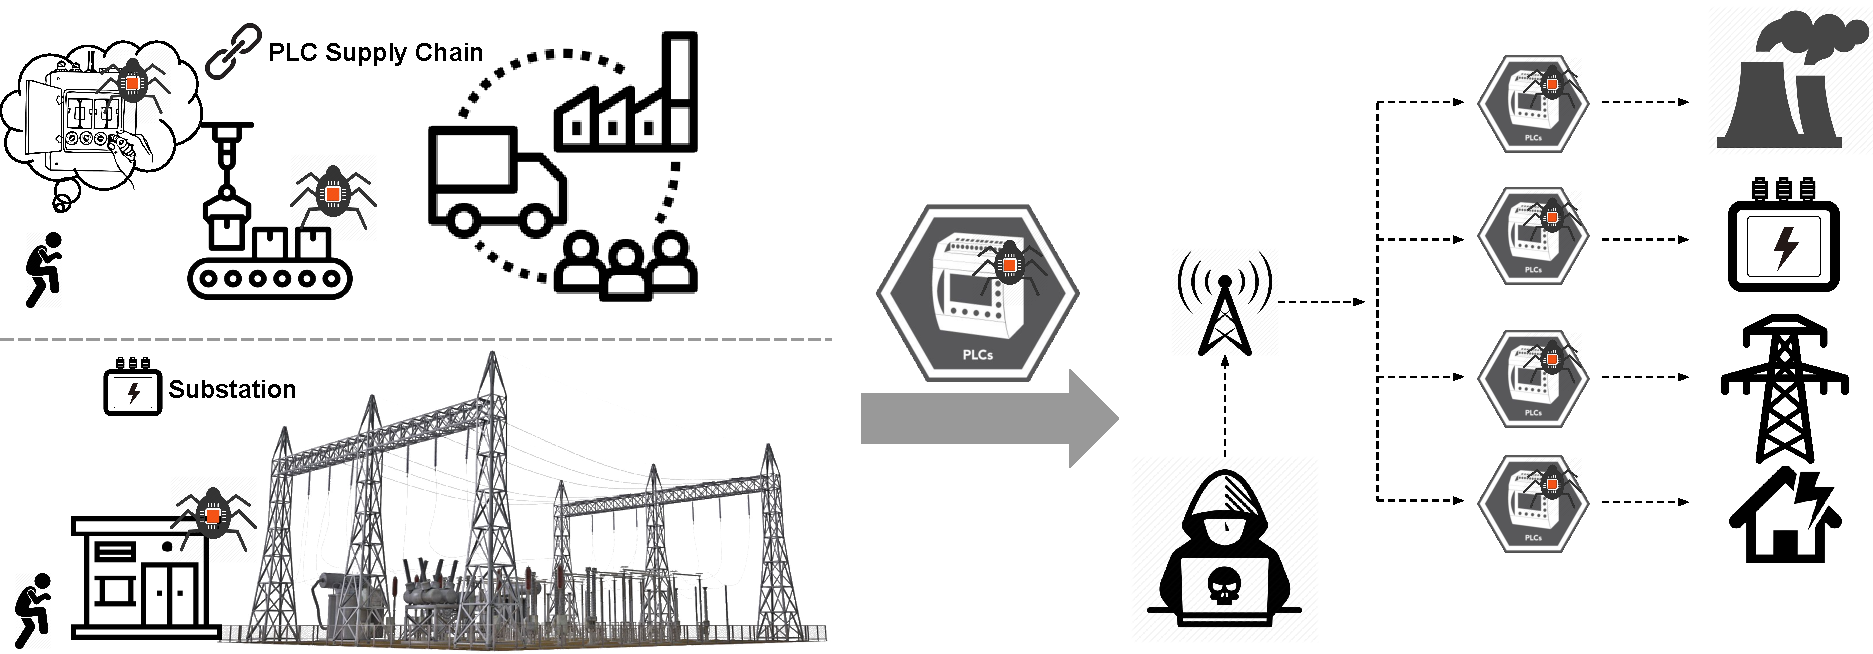
\includegraphics[width=\textwidth]{figures/bigpic}
	\centering
	\caption{In the PLC manufacturer factory or during the product shipment, numerous employees can access the PLCs. The hardware backdoor installation should follow specific procedures to be efficiently accomplished without advanced software knowledge. The hardware backdoor can communicate with the attacker through the GSM network. Therefore it does not need to join the ethernet used by the ICS system.}
	\label{fig:bigpic}
\end{figure*}


After the attacker controls enough PLCs, he can remotely initiate a distributed attack to cause more significant damage using a cellular network. 

The advantage of this attack is that it does not rely on the existing ICS network, nor is it limited to the firmware running on PLCs so that it can evade most software-based mitigations. It only needs to know the specific PLC model of the target and modify the hardware implant accordingly.



\subsection{Adversary Model}


The attacker knows the target's specific PLC model and can obtain the exact model for studying.

The printed circuit board (PCB) and the IC chips of the PLC should be well exposed. For example, the Chip-on-Board (COB)~\cite{lau1994chip} packing brings extra challenges for the attacker. The black glob-top makes it no easy to identify the chip model and pins. Fortunately, high-end microcontroller products rarely use this packaging. It would be a great advantage that the attacker can use the JTAG interface of the microcontroller.  In other words, the JTAG interface is not disabled by programming fusing bits at the factory. Nevertheless, the attacker can control the IO or tamper with the firmware image when transferred through the bus without JTAG.

To remotely control the device, the attacker uses a GSM network or WIFI to communicate with the hardware backdoor. The PLC must not be deployed in an electromagnetic isolation environment where the wireless signal can not be transmitted outside.

The operating system and software mitigation that runs on the microcontroller does not affect the backdoor. Therefore the PLC system allows having any memory protection based on MMU~\cite{shalan2000dynamic} and MPU~\cite{kim2018securing}.


\subsection{Challenges and Approaches}

The major challenge in attacking PLCs is not having enough information about the device. Some vendors publish the microcontroller's datasheet, but some vendors use proprietary design with highly customized instruction set architecture (ISA).  The layout of the PCB board and the on-board pin definition are also not publicly available.


\textbf{\textit{Firmware.}} In an embedded system, flash memory usually stores a file system and a real-time operating system (RTOS) such as VxWorks~\cite{neugass1991vxworks}. It is the so-called firmware. Specific to a real-time microcontroller, the firmware runs bare-metally on the microcontroller or with a lightweight RTOS such as FreeRTOS~\cite{barry2008freertos}. The PLC we use in this project is Allen Bradley 1769-L18ER-BBIB CompactLogix 5370. Through JTAG, we read the flash and ROM memory out of the microcontroller.
Moreover, we also ported a driver to read an on-board SPI flash chip, namely, AT45DB021. The source code is available at the github~\footnote{https://github.com/whensungoesdown/at45db021\_teensy32}.  We can identify the PLC use's internal data structures and libraries used with some reverse engineering effort.


\textbf{\textit{JTAG Pins.}} On some boards, the JTAG pins are difficult to trace, mainly when the microcontroller chip uses BGA packaging~\cite{joshi2000mosfet} that all the balls are buried underneath. In our case, there is a 10-pin solder pad, as shown in ~\autoref{fig:board-jtag}, which is likely to be an unsoldered JTAG socket (we also own one PLC that the socket is soldered on).  To identify each pin, we use a multimeter to conduct the connectivity test. The microcontroller supports both JTAG and Serial Wire Debug (SWD)\cite{ashfieldserial} interfaces.


\begin{figure}[th]
	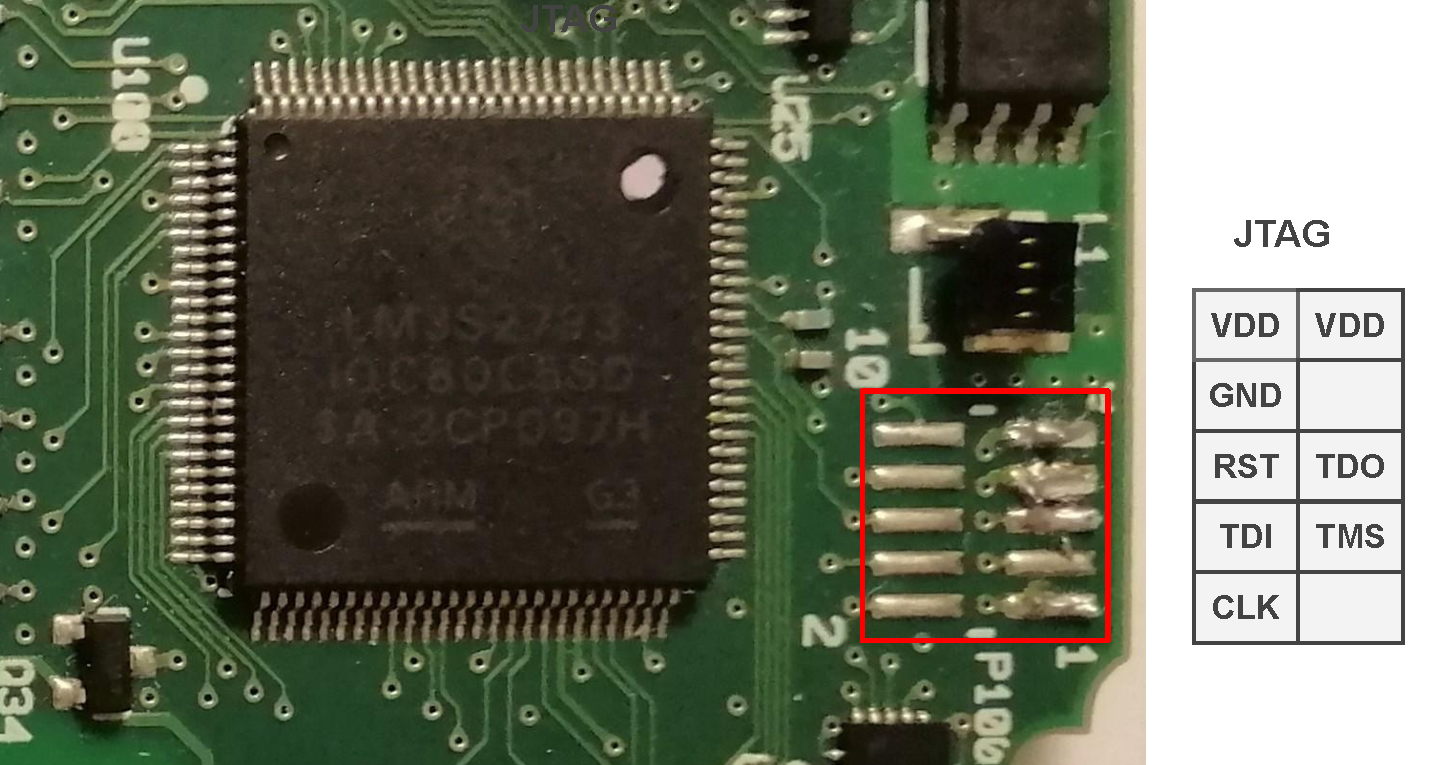
\includegraphics[width=0.47\textwidth]{figures/board-jtag}
	\centering
	\caption{JTAG pins on the real-time microcontroller board. A square pad with ten pins is very likely to be a JTAG interface. We need at least to have the TDI, TDO, TMS, and CLK. RST is optional.}
	\label{fig:board-jtag}
\end{figure}



\textbf{\textit{JTAG Protocol.}} To make our hardware backdoor small, we use the Teensy 3.2 development board. We also code a driver to send JTAG commands, hence accessing the microcontroller's on-chip resource. It is the equivalent of a trivial hardware debugger. Although the open-sourced debugger OpenOCD~\cite{hogl2006open} supports many platforms, the Cortex-M3 core that the Teensy has can not support its runtime environment. Our driver runs bare-metally on the microcontroller with minimal resource usage, and it can be ported to an even more restrained embedded system.  We also consider it as one of the paper's contributions. The source code is available at the github~\footnote{https://github.com/whensungoesdown/teensy\_jtag}. 


\textbf{\textit{Remote Control}} is a core function of the hardware backdoor. To avoid existing access control and even penetrate an air-gapped network, we use the SIM800C module to communicate with the backdoor through a separate GSM network.  It connects with the Teensy board using a serial port.

